\noindent A series of fast VCTs with test scenarios as listed in \autoref{tab:VCT_optiwise} were conducted with CFD in Shipflow \citep{alexanderssonVirtualCaptiveTests2017}. Rudder force predictions with the MMG original rudder model and the modified MMG quadratic model were compared to VCT data for the rudder angle variation as shown in \autoref{fig:rudder_angle_compare_optiwise}. The newly added initial inflow angle parameter $\gamma_0$ (see \autoref{eq:gamma_R2}) allows the MMG quadratic model to be better adapted to the VCT data. However, the difference between the models is less obvious when looking at the thrust variation tests in \autoref{fig:rudder_angle_compare_optiwise_all}.
%gamma_0, thrust_variation
\begin{figure}[h]
     \centering
     \begin{subfigure}[b]{0.49\textwidth}
         \centering
         \includesvg{figures/results_optiwise_VCT.rudder_angle.svg}
        \caption{Rudder angle variation.}
        \label{fig:rudder_angle_compare_optiwise}
     \end{subfigure}
     \hfill
     \begin{subfigure}[b]{0.49\textwidth}
         \centering
         \includesvg{figures/results_optiwise_VCT.thrust_variation.svg}
        \caption{Thrust variation at \textpm 10 degrees rudder angle.}
        \label{fig:thrust_variation_optiwise}
     \end{subfigure}
    \caption{Rudder angle variation and thrust variation.}
    \label{fig:rudder_angle_compare_optiwise_all}
\end{figure}
\FloatBarrier

The results of the drift, circle tests and the circle and drift tests are used to validate the MMG model improved by this study (named the MMG quadratic) for the prediction of the rudder forces.
The newly added quadratic relationship for the flow straightening coefficient $\gamma_R$ (\autoref{eq:gamma_R2}) in the MMG quadratic rudder model fits better to the VCT data than the original MMG rudder model, as shown in \autoref{fig:MMG_quadratic}.
%beta_R
\begin{figure}[h]
     \centering
     \begin{subfigure}[b]{0.49\textwidth}
         \centering
         \includesvg{figures/results_optiwise_VCT.Y_R_MMG_original.svg}
        \caption{Original MMG rudder model.}
        \label{fig:Y_R_MMG_original}
     \end{subfigure}
     \hfill
     \begin{subfigure}[b]{0.49\textwidth}
         \centering
         \includesvg{figures/results_optiwise_VCT.Y_R_MMG_quadratic.svg}
        \caption{Modified quadratic MMG rudder model.}
        \label{fig:Y_R_MMG_quadratic}
     \end{subfigure}
    \caption{Rudder force during the VCT tests as a function of the effective inflow angle for the original MMG model and the modified quadratic MMG model.}
    \label{fig:MMG_quadratic}
\end{figure}

The side force generated both on the rudder and the hull surface during various VCT analyses as listed in Table \ref{tab:VCT_optiwise} were used to validate the identified manoeuvring model by the proposed procedure for the Optiwise as in \autoref{fig:VCT_optiwise}. The results of the side forces for various rudder angle tests are presented in \autoref{fig:rudder_angle_X_optiwise} -- \autoref{fig:rudder_angle_N_optiwise}, where all the forces are well predicted by the model through the rudder hull interaction coefficients $x_R$ and $a_R$. 
The model predicts zero rudder drag when the rudder angle is zero at straight ahead condition as shown in \autoref{fig:rudder_angle_X_optiwise}. This is because the MMG rudder model has no base drag coefficient like the semi-empirical rudder model for the wPCC (see \autoref{fig:drift_angle_X_wPCC}).
Similar comparisons are shown for the drift angle tests in \autoref{fig:drift_angle_X_optiwise} -- \autoref{fig:drift_angle_N_optiwise} and the circle tests in \autoref{fig:circle_X_optiwise} -- \autoref{fig:circle_N_optiwise}. 
\begin{figure}[h]
    \centering
    %Rudder angle
    \begin{subfigure}[b]{0.325\textwidth}
         \centering
         \includesvg[width=1.2 in]{figures/results_optiwise_VCT.rudder_angle_X.svg}
        \caption{X for Rudder angle tests}
        \label{fig:rudder_angle_X_optiwise}
    \end{subfigure}
    \hfill
    \begin{subfigure}[b]{0.325\textwidth}
        \centering
        \includesvg{figures/results_optiwise_VCT.rudder_angle_Y.svg}
       \caption{Y for Rudder angle tests}
       \label{fig:rudder_angle_Y_optiwise}
    \end{subfigure}
    \hfill
    \begin{subfigure}[b]{0.325\textwidth}
        \centering
        \includesvg{figures/results_optiwise_VCT.rudder_angle_N.svg}
       \caption{N for Rudder angle tests}
       \label{fig:rudder_angle_N_optiwise}
    \end{subfigure}

    \vfill
    %Drift angle
    \begin{subfigure}[b]{0.325\textwidth}
        \centering
        \includesvg{figures/results_optiwise_VCT.drift_angle_X.svg}
       \caption{X for Drift angle tests}
       \label{fig:drift_angle_X_optiwise}
    \end{subfigure}
    \hfill
    \begin{subfigure}[b]{0.325\textwidth}
        \centering
        \includesvg{figures/results_optiwise_VCT.drift_angle_Y.svg}
       \caption{Y for Drift angle tests}
       \label{fig:drift_angle_Y_optiwise}
    \end{subfigure}
    \hfill
    \begin{subfigure}[b]{0.325\textwidth}
        \centering
        \includesvg{figures/results_optiwise_VCT.drift_angle_N.svg}
       \caption{N for Drift angle tests}
       \label{fig:drift_angle_N_optiwise}
    \end{subfigure}
    
    \vfill
    %Circle
    \begin{subfigure}[b]{0.325\textwidth}
        \centering
        \includesvg{figures/results_optiwise_VCT.circle_X.svg}
       \caption{X for Circle tests}
       \label{fig:circle_X_optiwise}
    \end{subfigure}
    \hfill
    \begin{subfigure}[b]{0.325\textwidth}
        \centering
        \includesvg{figures/results_optiwise_VCT.circle_Y.svg}
       \caption{Y for Circle tests}
       \label{fig:circle_Y_optiwise}
    \end{subfigure}
    \hfill
    \begin{subfigure}[b]{0.325\textwidth}
        \centering
        \includesvg{figures/results_optiwise_VCT.circle_N.svg}
       \caption{N for Circle tests}
       \label{fig:circle_N_optiwise}
    \end{subfigure}
    
    \caption{Forces on the Optiwise analyzed by VCT (dots) and predictions from the identified model (lines).}
    \label{fig:VCT_optiwise}
\end{figure}
\FloatBarrier

\vspace{-0.5cm}
It should also be noted that the coupling terms $Y_{vrr}$,$Y_{vvr}$,$N_{vrr}$, and $N_{vvr}$ play an important role in accurately modeling the forces. As shown in \autoref{fig:circle_drift_optiwise}, by considering those coupling terms, the sway forces and yaw moments obtained from the identified model give better results than no-coupling models for those circle and drift captive tests.
\begin{figure}[ht]
    \centering
    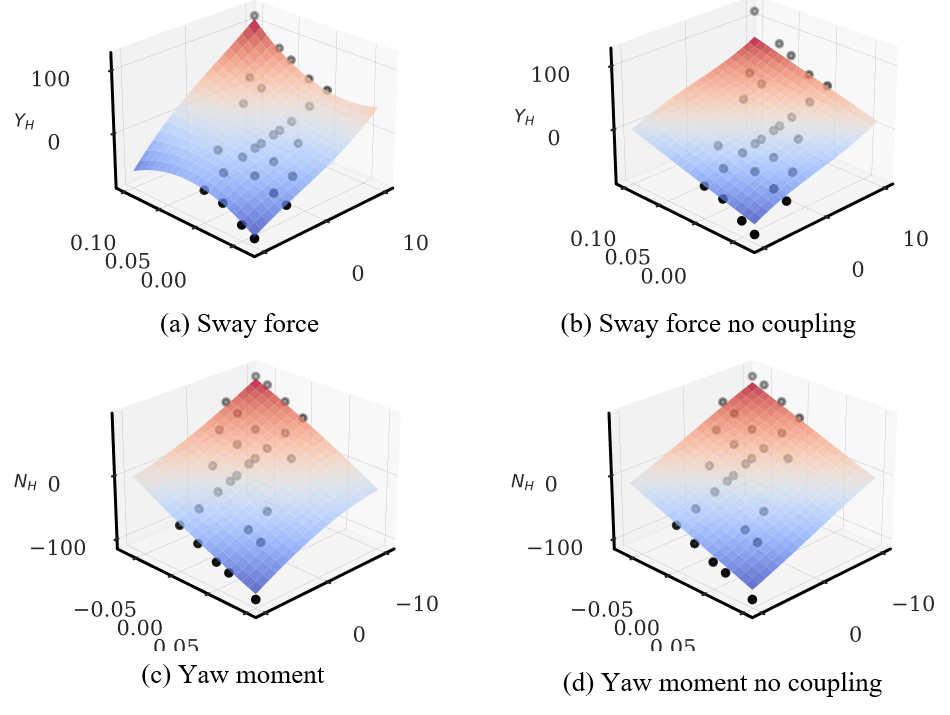
\includegraphics[width=0.7\linewidth]{figures/results_optiwise_vct.YNH.png}
    \caption{Optiwise hull forces during the circle and drift variations with/without the coupling terms, VCT (dots), fitted model (surface).}
    \label{fig:circle_drift_optiwise}
\end{figure}
\FloatBarrier

% % Circle + drift
% \begin{figure}[h]
%      \centering
%      \begin{subfigure}[b]{0.49\textwidth}
%          \centering
%          \includesvg{figures/results_optiwise_VCT.Y_H.svg}
%         \caption{Sway force.}
%         \label{fig:circle_drift_Y_H_optiwise}
%      \end{subfigure}
%      \hfill
%      \begin{subfigure}[b]{0.49\textwidth}
%          \centering         \includesvg{figures/results_optiwise_VCT.Y_H_no_coupling.svg}
%         \caption{Sway force no coupling.}
%         \label{fig:circle_drift_Y_H_no_coupling_optiwise}
%      \end{subfigure}
     
%      \vfill
%      \begin{subfigure}[b]{0.49\textwidth}
%          \centering
%          \includesvg{figures/results_optiwise_VCT.N_H.svg}
%         \caption{Yawing moment.}
%         \label{fig:circle_drift_N_H_optiwise}
%      \end{subfigure}
%      \hfill
%      \begin{subfigure}[b]{0.49\textwidth}
%          \centering
%          \includesvg{figures/results_optiwise_VCT.N_H_no_coupling.svg}
%         \caption{Yawing moment no coupling.}
%         \label{fig:circle_drift_N_H_no_coupling_optiwise}
%      \end{subfigure}
     
%     \caption{Optiwise hull forces during the circle and drift variations with/without the coupling terms, VCT (dots), fitted model (surface).}
%     \label{fig:circle_drift_optiwise}
% \end{figure}